% Provenance (never printed): cycle 4 SVT, "La planete Terre": earthquakes,
% faults, seismic waves and their recording, magnitude and intensity, the
% link with plate boundaries; natural hazards (tsunamis) and prevention; see
% sources/book1/PROVENANCE.md. Book 1, grade 7, chapter 3.
% Vocabulary guard: P and S waves are named in prose only (they were named in
% g6.4, defined in Book 2 g11); "sediment" not before g7.4; "intensity" is
% always the earthquake's (homograph with physics: linker STOP list).
\chapter{भूकंप}\label{ch:g7:earthquakes}

26~दिसंबर 2004 की सुबह, इंडोनेशिया में सुमात्रा के उत्तर-पश्चिमी सिरे के पास
\omterm{def:g2:water-on-earth:ocean}{समुद्र} के नीचे, \omterm{def:g3:stones-pebbles-sand:rock}{चट्टानें} एक \omterm{def:g7:earthquakes:fault}{भ्रंश} के साथ टूट गईं: यह अब तक मापे गए सबसे बड़े
\omterm{def:g4:volcanoes-earthquakes-first-look:earthquake}{भूकंपों} में से एक था। सुमात्रा के पास के \omterm{def:g1:landscapes-around-us:water}{तट} पर \omterm{def:g2:water-on-earth:ocean}{समुद्र} \qty{51}{m} तक ऊँची लहरों
में उठा, जो ज़मीन के अंदर \qty{5}{km} तक बह गईं। अगले घंटों में लहरों ने हिंद
\omterm{def:g2:water-on-earth:ocean}{महासागर} पार किया और पंद्रह देशों के तटों से टकराईं, अफ़्रीका तक। लगभग
230\,000 लोग मारे गए। उस समय हिंद \omterm{def:g2:water-on-earth:ocean}{महासागर} में कोई चेतावनी प्रणाली नहीं
थी।
% ledger: usgs:largest, nws:tsunami-2004

\begin{omfigure}
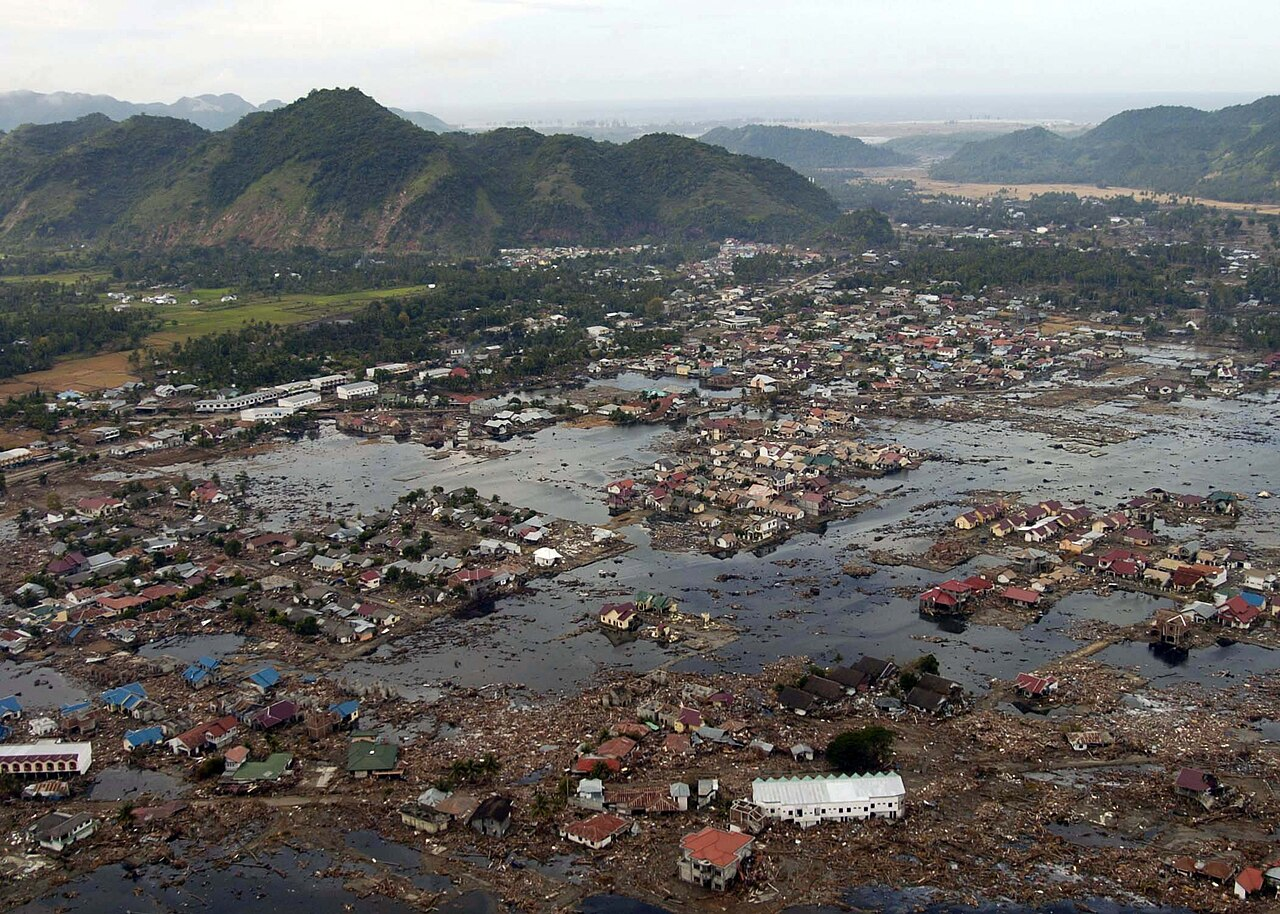
\includegraphics[width=0.78\linewidth]{images/book1/g7-tsunami-village.jpg}

{\small \omterm{def:g7:earthquakes:tsunami}{सुनामी} के एक हफ़्ते बाद, 26~दिसंबर 2004, सुमात्रा के \omterm{def:g1:landscapes-around-us:water}{तट} के पास का एक गाँव।
अमेरिकी नौसेना की फ़ोटो, फ़िलिप मैकडैनियल द्वारा (सार्वजनिक डोमेन, विकिमीडिया
कॉमन्स के ज़रिए)।}
% ledger: commons:tsunami-village
\label{fig:g7:earthquakes:tsunami-village}
\end{omfigure}

\omterm{def:g3:stones-pebbles-sand:rock}{चट्टानें} कैसे टूटती हैं? वैज्ञानिक कुछ ही मिनटों में कैसे पता कर लेते हैं कि \omterm{def:g4:volcanoes-earthquakes-first-look:earthquake}{भूकंप}
कहाँ आया और कितना बड़ा था? और घंटों बाद \omterm{def:g2:water-on-earth:ocean}{समुद्र} उन तटों पर क्यों उठा जहाँ किसी ने
कुछ भी महसूस नहीं किया था?

\begin{recall}
\emph{\omterm{def:g4:volcanoes-earthquakes-first-look:earthquake}{भूकंप}} ज़मीन का अचानक काँपना है, जो ज़मीन के बहुत नीचे \omterm{def:g3:stones-pebbles-sand:rock}{चट्टानों} के टूटने और
फिसलने से होता है (\cref{ch:g4:volcanoes-earthquakes-first-look})। पृथ्वी का
बाहरी कवच \omterm{def:g7:plate-tectonics:plate}{प्लेटों} से बना है, और 92~\% बड़े \omterm{def:g4:volcanoes-earthquakes-first-look:earthquake}{भूकंप} किसी \omterm{def:g7:plate-tectonics:plate-boundary}{प्लेट सीमा} से
\qty{300}{km} से कम दूरी पर आते हैं (\cref{ch:g7:plate-tectonics})। जब \omterm{def:g4:volcanoes-earthquakes-first-look:earthquake}{भूकंप} आता
है, तो पूरी पृथ्वी की \omterm{def:g3:stones-pebbles-sand:rock}{चट्टानों} में से तरंगें गुज़रती हैं: एक तेज़ प्रकार की
(P~तरंगें) और एक धीमे प्रकार की (S~तरंगें); उनका समय मापकर वैज्ञानिकों ने \omterm{def:g6:inside-the-earth:layers}{क्रोड}
की खोज की
(\cref{ch:g6:inside-the-earth})।
\end{recall}

\section{टूटती चट्टानें}

\omterm{def:g7:plate-tectonics:plate}{प्लेटें} साल में कुछ सेंटीमीटर चलती हैं, पर उनके किनारे खुरदुरे होते हैं: वे आपस में
चिपके रहते हैं जबकि \omterm{def:g7:plate-tectonics:plate}{प्लेटों} का बाकी हिस्सा चलता रहता है। किनारे के पास की \omterm{def:g3:stones-pebbles-sand:rock}{चट्टानें}
थोड़ी मुड़ती हैं, उस पटरी की तरह जिसे तुम दोनों सिरों से दबाते हो, और ऊर्जा जमा
करती हैं। जब धक्का आख़िरकार घर्षण पर भारी पड़ता है, तो \omterm{def:g3:stones-pebbles-sand:rock}{चट्टानें} एक साथ छूटकर
फिसल जाती हैं: वह अचानक फिसलन ही \omterm{def:g4:volcanoes-earthquakes-first-look:earthquake}{भूकंप} है।
% ledger: usgs:eq-basics

\begin{definition}[भ्रंश]\label{def:g7:earthquakes:fault}
\emph{भ्रंश}\index{भ्रंश} \omterm{def:g3:stones-pebbles-sand:rock}{चट्टानों} में एक दरार है जिसके साथ-साथ दोनों ओर के खंड
एक-दूसरे के सापेक्ष खिसके हैं। \omterm{def:g4:volcanoes-earthquakes-first-look:earthquake}{भूकंप} के दौरान खंड भ्रंश के साथ-साथ अचानक फिसलते
हैं; भ्रंश और फिसलन जितने बड़े, \omterm{def:g4:volcanoes-earthquakes-first-look:earthquake}{भूकंप} उतना ही
बड़ा।
\end{definition}

\omterm{def:g7:plate-tectonics:plate-boundary}{प्लेट सीमा} बहुत-से \omterm{def:g7:earthquakes:fault}{भ्रंशों} से बनी होती है, और दुनिया के ज़्यादातर \omterm{def:g4:volcanoes-earthquakes-first-look:earthquake}{भूकंप} उन्हीं पर
आते हैं। पर \omterm{def:g7:earthquakes:fault}{भ्रंश} \omterm{def:g7:plate-tectonics:plate}{प्लेटों} के अंदर भी होते हैं, और उनमें से कुछ भी टूट सकते हैं। जब
कोई बड़ा \omterm{def:g7:earthquakes:fault}{भ्रंश} सतह के पास टूटता है, तो फिसलन ज़मीन पर दिख सकती है: किसी खेत में एक
सीढ़ी-सा उभार, दो हिस्सों में कटी सड़क, एक तरफ़ खिसकी बाड़ या पेड़ों की
कतार।
% ledger: usgs:eq-basics

\begin{omfigure}
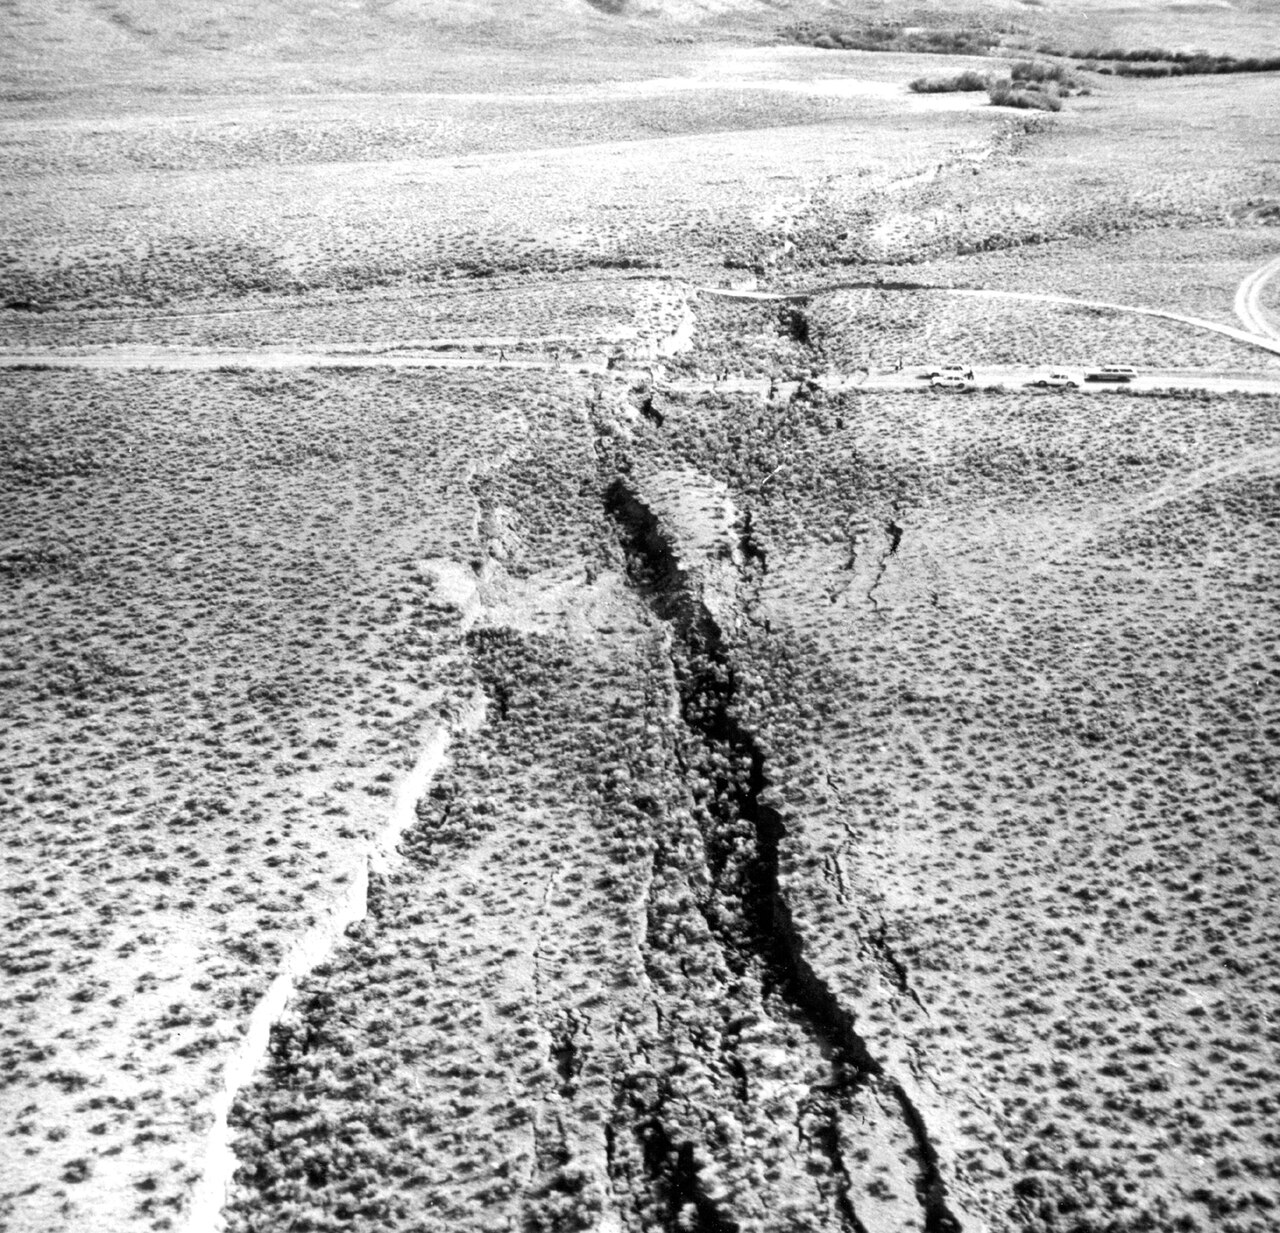
\includegraphics[width=0.62\linewidth]{images/book1/g7-borah-scarp.jpg}

{\small 1983 के बोरा पीक \omterm{def:g4:volcanoes-earthquakes-first-look:earthquake}{भूकंप} के बाद आइडाहो (संयुक्त राज्य अमेरिका) में ज़मीन पर
बचे सीढ़ीनुमा उभार, हवा से: \omterm{def:g7:earthquakes:fault}{भ्रंश} के साथ-साथ एक ओर का हिस्सा दूसरी ओर के सापेक्ष
नीचे बैठ गया, और यह उभार ऊपर वाली सड़क को काटता है। फ़ोटो: वॉलेस, अमेरिकी
भूवैज्ञानिक सर्वेक्षण (सार्वजनिक डोमेन,
विकिमीडिया कॉमन्स के ज़रिए)।}
% ledger: commons:borah-scarp
\label{fig:g7:earthquakes:borah}
\end{omfigure}

\begin{definition}[भूकंप-मूल और अधिकेंद्र]\label{def:g7:earthquakes:focus}
किसी \omterm{def:g4:volcanoes-earthquakes-first-look:earthquake}{भूकंप} का \emph{भूकंप-मूल}\index{भूकंप-मूल} ज़मीन के नीचे, \omterm{def:g7:earthquakes:fault}{भ्रंश} पर, वह जगह
है जहाँ फिसलन शुरू होती है। \emph{अधिकेंद्र}\index{अधिकेंद्र} पृथ्वी की सतह पर
भूकंप-मूल के ठीक ऊपर वाला बिंदु है।
\end{definition}

\omterm{def:g7:earthquakes:focus}{भूकंप-मूल} अक्सर कुछ किलोमीटर से लेकर कुछ दसियों किलोमीटर तक गहरा होता है। 1976
और 2025 के बीच दर्ज \omterm{def:g7:earthquakes:magnitude}{परिमाण}~6 या उससे ज़्यादा के 7\,031 \omterm{def:g4:volcanoes-earthquakes-first-look:earthquake}{भूकंपों} में से 5\,561 ---
79~\% --- का \omterm{def:g7:earthquakes:focus}{भूकंप-मूल} \qty{70}{km} से कम गहराई पर था। पर 483 \omterm{def:g4:volcanoes-earthquakes-first-look:earthquake}{भूकंप}
\qty{300}{km} से ज़्यादा गहराई पर शुरू हुए, और सबसे गहरा
\qty{688}{km} नीचे: ये गहरे \omterm{def:g4:volcanoes-earthquakes-first-look:earthquake}{भूकंप} वहाँ आते हैं जहाँ एक \omterm{def:g7:plate-tectonics:plate}{प्लेट} दूसरी के नीचे धँसती
है, धँसती \omterm{def:g7:plate-tectonics:plate}{प्लेट} के अंदर।
% ledger: data:usgs-comcat (figdata/grade-7/quake_counts.py, part depth)

बड़ा \omterm{def:g4:volcanoes-earthquakes-first-look:earthquake}{भूकंप} शायद ही कभी अकेला आता है। अक्सर उसके बाद उसी जगह पर छोटे \omterm{def:g4:volcanoes-earthquakes-first-look:earthquake}{भूकंप} आते
हैं, \emph{पश्च-आघात}, हफ़्तों, महीनों और यहाँ तक कि वर्षों तक। कभी-कभी उससे पहले
छोटे \omterm{def:g4:volcanoes-earthquakes-first-look:earthquake}{भूकंप} आते हैं, पर बड़ा \omterm{def:g4:volcanoes-earthquakes-first-look:earthquake}{भूकंप} आ जाने तक कोई नहीं बता सकता कि वे चेतावनियाँ
थीं: वैज्ञानिक \omterm{def:g4:volcanoes-earthquakes-first-look:earthquake}{भूकंपों} की भविष्यवाणी नहीं कर सकते। वे केवल यह बता सकते हैं कि
कौन-से \omterm{def:g7:earthquakes:fault}{भ्रंश} किसी दिन फिर टूटेंगे, और लोगों को तैयार होने में मदद कर
सकते हैं।
% ledger: usgs:eq-basics, usgs:seismograph

\begin{omfigure}
\begin{tikzpicture}[font=\small, x=1cm, y=1cm]
  % a block of crust seen in perspective: front face and top face
  \def\dx{2.2}\def\dy{1.3}
  % top surface: two blocks separated by the fault trace
  \fill[green!12] (0,0) -- (4.6,0) -- (4.6+\dx,\dy) -- (\dx,\dy) -- cycle;
  \fill[green!18] (4.6,0) -- (9,0) -- (9+\dx,\dy) -- (4.6+\dx,\dy) -- cycle;
  % front face
  \fill[brown!30] (0,0) -- (4.6,0) -- (3.4,-4) -- (0,-4) -- cycle;
  \fill[brown!40] (4.6,0) -- (9,0) -- (9,-4) -- (3.4,-4) -- cycle;
  % right face
  \fill[brown!22] (9,0) -- (9+\dx,\dy) -- (9+\dx,\dy-4) -- (9,-4) -- cycle;
  % fault plane on the front face and trace on top
  \draw[very thick, red!70!black] (4.6,0) -- (3.4,-4);
  \draw[very thick, red!70!black] (4.6,0) -- (4.6+\dx,\dy);
  % slip arrows
  \draw[-{Stealth[length=2.5mm]}, thick] (2.6,-0.35) -- (1.6,-0.35);
  \draw[-{Stealth[length=2.5mm]}, thick] (6.4,-0.35) -- (7.4,-0.35);
  \node[font=\footnotesize, anchor=south] at (2.1,-0.3) {खंड 1};
  \node[font=\footnotesize, anchor=south] at (6.9,-0.3) {खंड 2};
  % focus and waves
  \coordinate (F) at (3.95,-2.4);
  \foreach \r in {0.5,1.0,1.5,2.0}
    \draw[blue!60, dashed] (F) circle (\r);
  \fill[red!80!black] (F) circle (0.13);
  % epicentre: on the surface, straight above the focus (front edge of the top face)
  \coordinate (E) at (3.95,0);
  \draw[black!60, densely dotted, thick] (F) -- (E);
  \node[star, star points=5, star point ratio=2.4, fill=orange, draw=black, inner sep=1.4pt] at (E) {};
  % labels
  \node[anchor=west] at (9.5,-2.3) {भूकंप-मूल};
  \draw[black!60] (9.45,-2.3) -- (4.1,-2.4);
  \node[anchor=south west] at (4.9,1.9) {अधिकेंद्र};
  \draw[black!60] (4.95,1.95) -- (4.05,0.12);
  \node[anchor=south, red!70!black] at (6.8,1.3) {भ्रंश};
  \node[anchor=east, blue!60!black, align=right] at (-0.15,-2.6) {तरंगें सभी\\दिशाओं में फैलती हैं};
  \draw[blue!60, -{Stealth}] (-0.1,-2.6) -- (1.9,-2.5);
\end{tikzpicture}

{\small एक \omterm{def:g7:earthquakes:fault}{भ्रंश}, \omterm{def:g7:earthquakes:focus}{भूकंप-मूल} और \omterm{def:g7:earthquakes:focus}{अधिकेंद्र} (एक चित्र, पैमाने पर नहीं)। दोनों खंड
\omterm{def:g7:earthquakes:fault}{भ्रंश} (लाल) के साथ-साथ एक-दूसरे के पास से फिसलते हैं; फिसलन \omterm{def:g7:earthquakes:focus}{भूकंप-मूल} पर शुरू
होती है, और उससे तरंगें सभी दिशाओं में फैलती हैं, जैसे तालाब में लहरें।
\omterm{def:g7:earthquakes:focus}{अधिकेंद्र} (तारा) सतह पर, \omterm{def:g7:earthquakes:focus}{भूकंप-मूल} के ठीक ऊपर
है।}
% ledger: usgs:eq-basics
\label{fig:g7:earthquakes:fault}
\end{omfigure}


\section{भूकंप को दर्ज करना}

\begin{definition}[भूकंपमापी और भूकंपलेख]\label{def:g7:earthquakes:seismometer}
\emph{भूकंपमापी}\index{भूकंपमापी} एक उपकरण है जो ज़मीन के काँपने को दर्ज करता
है। उसका रिकॉर्ड, समय के सापेक्ष बनी एक लहरदार रेखा,
\emph{भूकंपलेख}\index{भूकंपलेख} है।
\end{definition}

\omterm{def:g7:earthquakes:seismometer}{भूकंपमापी} का विचार सरल है। एक ढाँचा ज़मीन से मज़बूती से जुड़ा है; उससे एक स्प्रिंग
पर एक भारी वज़न लटका है। जब ज़मीन काँपती है, तो ढाँचा उसके साथ काँपता है, पर भारी
वज़न, जिसे केवल उसकी स्प्रिंग थामे है, लगभग स्थिर रहता है। उपकरण स्थिर वज़न के
सापेक्ष ढाँचे की गति दर्ज करता है: यही ज़मीन की गति है। नीचे के चित्र में द्रव्यमान
से जुड़ी एक क़लम उसे घूमते ड्रम पर लिपटे काग़ज़ पर
बनाती है।
% ledger: usgs:seismograph

\begin{omfigure}
\begin{tikzpicture}[font=\small, x=1cm, y=1cm]
  \begin{scope}
    % ground
    \fill[brown!30] (-0.6,-0.6) rectangle (5.0,0);
    \draw[decorate, decoration={snake, amplitude=1.2pt, segment length=6pt}, brown!70!black, thick]
      (-0.6,0) -- (5.0,0);
    % frame
    \fill[black!55] (0,0) rectangle (0.25,3.2);
    \fill[black!55] (0,3.0) rectangle (2.4,3.25);
    % spring and weight
    \draw[decorate, decoration={coil, aspect=0.5, segment length=3pt, amplitude=4pt}, thick]
      (2.1,3.0) -- (2.1,2.1);
    \fill[black!80] (1.7,1.45) rectangle (2.5,2.1);
    \node[white, font=\scriptsize] at (2.1,1.78) {भार};
    % pen arm and drum
    \draw[thick] (2.5,1.75) -- (3.45,1.75);
    \fill (3.45,1.75) circle (0.05);
    \draw[thick, fill=white] (3.95,1.75) circle (0.5);
    \draw[thick] (3.95,1.25) -- (3.95,0);
    \draw[-{Stealth}, black!60] (4.55,2.2) arc (40:-40:0.7);
    % labels
    \node[anchor=east, align=right, font=\footnotesize] at (-0.1,2.3) {ज़मीन से जुड़ा\\ढाँचा};
    \node[anchor=west, font=\footnotesize] at (2.6,2.65) {स्प्रिंग};
    \draw[black!60] (2.55,2.65) -- (2.25,2.6);
    \node[anchor=north, align=center, font=\footnotesize] at (2.1,1.35) {भारी द्रव्यमान:\\स्थिर रहता है};
    \node[anchor=west, align=left, font=\footnotesize] at (4.7,1.05) {घूमता ड्रम,\\उस पर\\काग़ज़};
    \node[anchor=north, font=\footnotesize] at (2.2,-0.65) {ज़मीन काँपती है};
  \end{scope}
  \begin{scope}[xshift=7.2cm, yshift=0.4cm]
    \begin{axis}[width=7.6cm, height=4.2cm, xmin=0, xmax=60, ymin=-1.1, ymax=1.1,
        axis x line=bottom, axis y line=none, xlabel={समय (सेकंड)},
        tick label style={font=\scriptsize}, label style={font=\footnotesize}, clip=false]
      \addplot[black, line width=0.4pt] table[x=t, y=v] {figdata/out/grade-7-epicentre-m-trace.dat};
      \draw[blue!70!black, -{Stealth[length=2mm]}] (axis cs:10,1.45) -- (axis cs:10,0.45);
      \node[blue!70!black, font=\scriptsize, anchor=south east] at (axis cs:10.5,1.45) {तेज़ तरंगें पहुँचती हैं};
      \draw[red!70!black, -{Stealth[length=2mm]}] (axis cs:20,1.45) -- (axis cs:20,1.05);
      \node[red!70!black, font=\scriptsize, anchor=south west] at (axis cs:19.5,1.45) {धीमी तरंगें पहुँचती हैं};
      \draw[{Stealth[length=2mm]}-{Stealth[length=2mm]}] (axis cs:10,-0.75) -- (axis cs:20,-0.75);
      \node[font=\scriptsize, anchor=east] at (axis cs:9,-0.75) {देरी: 10 सेकंड};
    \end{axis}
  \end{scope}
\end{tikzpicture}

{\small बाएँ: \omterm{def:g7:earthquakes:seismometer}{भूकंपमापी} का सिद्धांत (एक चित्र)। दाएँ: इस किताब के लिए बनाया गया
एक \omterm{def:g7:earthquakes:seismometer}{भूकंपलेख} (असली रिकॉर्ड नहीं): रेखा शांत है, फिर तेज़ तरंगें पहुँचती हैं, फिर
दस सेकंड बाद धीमी और बड़ी
तरंगें।}
% ledger: usgs:seismograph (trace drawn by figdata/grade-7/epicentre.py, part m-trace)
\label{fig:g7:earthquakes:seismometer}
\end{omfigure}

\subsection*{भूकंप कितनी दूर था?}

\omterm{def:g7:earthquakes:seismometer}{भूकंपलेख} ``ज़मीन काँपी'' से ज़्यादा बताता है। तेज़ तरंगें हमेशा पहले पहुँचती हैं
और धीमी बाद में। \omterm{def:g7:earthquakes:focus}{भूकंप-मूल} के पास वे लगभग साथ-साथ पहुँचती हैं; दूर, धीमी तरंगें
और ज़्यादा पीछे छूटती जाती हैं, ठीक वैसे ही जैसे \omterm{def:g5:natural-hazards:storm}{तूफ़ान} के दौरान, \omterm{def:g5:natural-hazards:storm}{तूफ़ान} दूर हो तो
गरज बिजली की चमक से ज़्यादा पीछे रह जाती है। इसलिए दोनों के पहुँचने के बीच की
देरी \omterm{def:g4:volcanoes-earthquakes-first-look:earthquake}{भूकंप} की दूरी बताती है।
% ledger: usgs:seismograph

देरी के हर सेकंड के लिए कितने किलोमीटर? यह इस पर निर्भर करता है कि दोनों तरंगें
जिन \omterm{def:g3:stones-pebbles-sand:rock}{चट्टानों} को पार करती हैं, उनमें उनकी चाल कितनी है। पृथ्वी के संदर्भ मॉडल की
चालों से (\cref{ch:g6:inside-the-earth}), देरी का हर सेकंड ऊपरी \omterm{def:g6:inside-the-earth:layers}{भूपर्पटी} में
लगभग \qty{7}{km} और निचली \omterm{def:g6:inside-the-earth:layers}{भूपर्पटी} में \qty{9}{km} दर्शाता है। इस अध्याय के
अभ्यासों में हम हर सेकंड के लिए \qty{8}{km} का गोल मान लेते
हैं।
% ledger: data:prem (computed in figdata/grade-7/epicentre.py, part rule)

\begin{method}[तीन स्टेशनों से अधिकेंद्र ढूँढना]\label{met:g7:earthquakes:three-circles}
\begin{enumerate}
  \item हर स्टेशन के \omterm{def:g7:earthquakes:seismometer}{भूकंपलेख} पर तेज़ तरंगों के पहुँचने और धीमी तरंगों के पहुँचने
        के बीच की देरी पढ़ो।
  \item हर देरी को दूरी में बदलो (यहाँ: सेकंड में देरी का $8 \times$, किलोमीटर
        में)।
  \item \omterm{def:g2:drawing-to-map:map}{मानचित्र} पर हर स्टेशन के चारों ओर एक वृत्त बनाओ जिसकी त्रिज्या उसकी दूरी
        हो। \omterm{def:g7:earthquakes:focus}{अधिकेंद्र} हर वृत्त पर कहीं न कहीं है।
  \item दो वृत्तों से आमतौर पर दो संभावित बिंदु मिलते हैं; तीसरा वृत्त उनमें से
        केवल एक से गुज़रता है: वही \omterm{def:g7:earthquakes:focus}{अधिकेंद्र} है।
\end{enumerate}
\end{method}

\begin{example}[तीन वृत्त]\label{ex:g7:earthquakes:three-circles}
तीन स्टेशन एक ही \omterm{def:g4:volcanoes-earthquakes-first-look:earthquake}{भूकंप} दर्ज करते हैं। देरियाँ स्टेशन~M1 पर \qty{10}{s},
M2 पर \qty{11.25}{s} और M3 पर \qty{9.75}{s} हैं। दूरियाँ
$8 \times 10 = \qty{80}{km}$, $8 \times 11.25 = \qty{90}{km}$ और
$8 \times 9.75 = \qty{78}{km}$ हैं। नीचे बने तीनों वृत्त एक ही बिंदु पर मिलते
हैं: \omterm{def:g7:earthquakes:focus}{अधिकेंद्र}।
% ledger: usgs:seismograph (figdata/grade-7/epicentre.py, parts m-stations and m-circles)
\end{example}

\begin{omfigure}
\begin{tikzpicture}
  \begin{axis}[axis equal image, width=8.2cm, xmin=-150, xmax=170, ymin=-160, ymax=160,
      xtick={-120,-80,...,160}, ytick={-120,-80,...,120}, grid=both, grid style={black!12},
      tick label style={font=\scriptsize}, xlabel={km}, ylabel={km}, label style={font=\footnotesize}]
    \addplot[blue!60!black, line width=0.6pt] table[x=x, y=y] {figdata/out/grade-7-epicentre-m-circles.dat};
    \addplot[only marks, mark=triangle*, mark size=3pt, black,
        nodes near coords, point meta=explicit symbolic,
        nodes near coords style={font=\scriptsize, anchor=north, yshift=-2pt}]
      table[x=x, y=y, meta=name] {figdata/out/grade-7-epicentre-m-stations.dat};
    \node[star, star points=5, star point ratio=2.4, fill=orange, draw=black, inner sep=1.6pt] at (axis cs:0,0) {};
    \draw[black!60] (axis cs:-4,-4) -- (axis cs:-60,-75);
    \node[font=\scriptsize, anchor=north east, inner sep=1pt] at (axis cs:-60,-75) {अधिकेंद्र};
  \end{axis}
\end{tikzpicture}

{\small हर वृत्त का केंद्र एक स्टेशन (त्रिकोण) पर है, और उसकी त्रिज्या \omterm{def:g4:volcanoes-earthquakes-first-look:earthquake}{भूकंप} से उस
स्टेशन की दूरी के बराबर है। तीनों वृत्त केवल एक बिंदु पर मिलते हैं, \omterm{def:g7:earthquakes:focus}{अधिकेंद्र}
(तारा)।}
% ledger: usgs:seismograph (figdata/grade-7/epicentre.py, parts m-stations and m-circles)
\label{fig:g7:earthquakes:three-circles}
\end{omfigure}

\begin{omfigure}
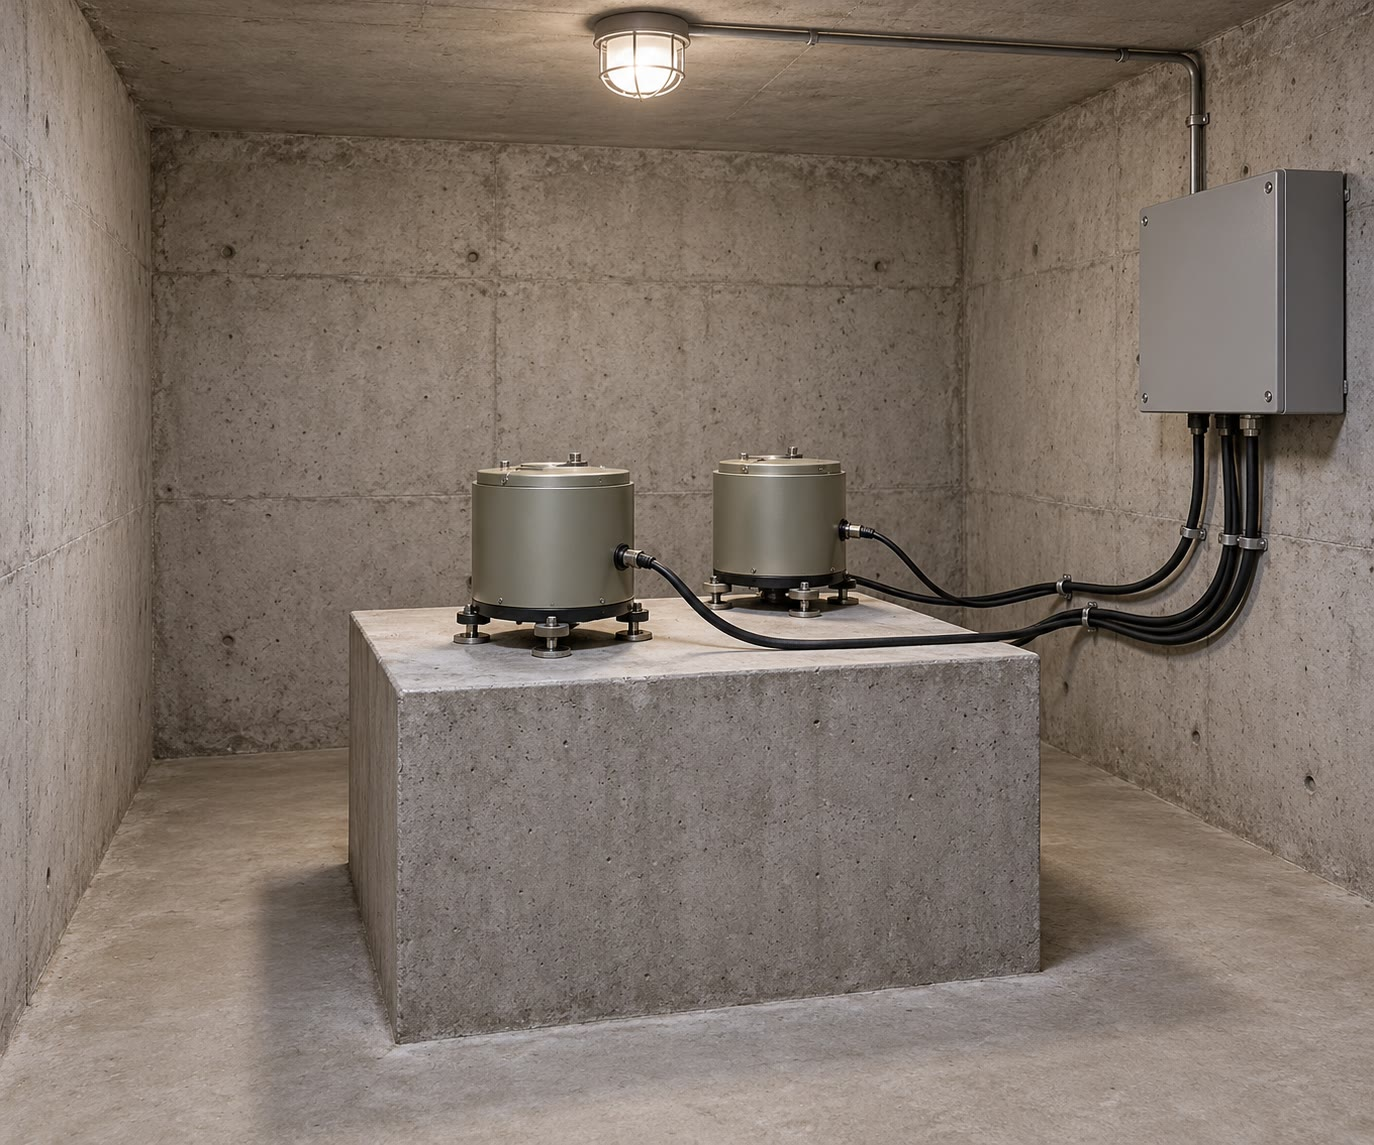
\includegraphics[width=0.58\linewidth]{images/book1/ai/g7-seismometer-vault.jpg}

{\small एक शांत भूमिगत कमरे में \omterm{def:g7:earthquakes:seismometer}{भूकंपमापी}, सड़कों और मशीनों से दूर, कंक्रीट के एक
चबूतरे पर रखे हुए जो \omterm{def:g3:stones-pebbles-sand:rock}{चट्टान} पर टिका है (एक सामान्य दृश्य का
AI चित्रण)।}
\label{fig:g7:earthquakes:vault}
\end{omfigure}

\section{कितना बड़ा? परिमाण और तीव्रता}

दो अलग-अलग संख्याएँ \omterm{def:g4:volcanoes-earthquakes-first-look:earthquake}{भूकंप} का वर्णन करती हैं, और उन्हें अक्सर आपस में मिला दिया जाता है।

\begin{definition}[परिमाण]\label{def:g7:earthquakes:magnitude}
किसी \omterm{def:g4:volcanoes-earthquakes-first-look:earthquake}{भूकंप} का \emph{परिमाण}\index{परिमाण} उसका आकार मापता है: स्रोत पर निकली
ऊर्जा। इसे \omterm{def:g7:earthquakes:seismometer}{भूकंपलेखों} से निकाला जाता है। हर \omterm{def:g4:volcanoes-earthquakes-first-look:earthquake}{भूकंप} का एक ही परिमाण होता है, जिसे
एक दशमलव स्थान के साथ लिखा जाता है, जैसे
6.3 या 9.1।
\end{definition}

\begin{definition}[तीव्रता]\label{def:g7:earthquakes:intensity}
किसी जगह पर \omterm{def:g4:volcanoes-earthquakes-first-look:earthquake}{भूकंप} की \emph{तीव्रता}\index{तीव्रता} बताती है कि वहाँ ज़मीन कितनी
ज़ोर से काँपी, लोगों ने जो महसूस किया और जो नुकसान देखा, उसके आधार पर। इसे रोमन
अंकों में लिखा जाता है, I (महसूस नहीं हुआ) से XII (पूरा विनाश) तक। एक \omterm{def:g4:volcanoes-earthquakes-first-look:earthquake}{भूकंप} की
बहुत-सी तीव्रताएँ होती हैं: हर जगह एक अलग
तीव्रता।
\end{definition}

\omterm{def:g7:earthquakes:magnitude}{परिमाण} का पैमाना तेज़ी से चढ़ता है। \omterm{def:g7:earthquakes:magnitude}{परिमाण} में 1 का हर क़दम \omterm{def:g7:earthquakes:seismometer}{भूकंपलेख} पर लगभग
10~गुना बड़ी तरंगें और लगभग 32~गुना ज़्यादा निकली ऊर्जा दर्शाता है। \omterm{def:g7:earthquakes:magnitude}{परिमाण}~8 का
\omterm{def:g4:volcanoes-earthquakes-first-look:earthquake}{भूकंप} \omterm{def:g7:earthquakes:magnitude}{परिमाण}~6 वाले से लगभग
$32 \times 32 \approx 1000$ गुना ज़्यादा ऊर्जा छोड़ता है।
% ledger: usgs:mag-energy

\begin{method}[दो परिमाणों की तुलना]\label{met:g7:earthquakes:magnitudes}
दो \omterm{def:g4:volcanoes-earthquakes-first-look:earthquake}{भूकंपों} की ऊर्जा की तुलना करने के लिए, उनके \omterm{def:g7:earthquakes:magnitude}{परिमाणों} के बीच पूरे क़दम गिनो, और
हर क़दम के लिए एक बार 32 से गुणा करो: 1~क़दम, 32~गुना; 2~क़दम, लगभग
1000~गुना; 3~क़दम, लगभग 32\,000~गुना।
\end{method}

\begin{example}[परिमाण 9 और परिमाण 7]\label{ex:g7:earthquakes:nine-seven}
2004 के सुमात्रा के पास वाले \omterm{def:g4:volcanoes-earthquakes-first-look:earthquake}{भूकंप} का \omterm{def:g7:earthquakes:magnitude}{परिमाण} 9.1 था। \omterm{def:g7:earthquakes:magnitude}{परिमाण}~7.1 का \omterm{def:g4:volcanoes-earthquakes-first-look:earthquake}{भूकंप} दो
क़दम छोटा है: उसने लगभग
$32 \times 32 = 1024$, यानी लगभग 1000~गुना, कम ऊर्जा छोड़ी।
% ledger: usgs:largest, usgs:mag-energy
\end{example}

अब तक मापे गए सबसे बड़े \omterm{def:g4:volcanoes-earthquakes-first-look:earthquake}{भूकंप} सभी वहाँ आए जहाँ एक \omterm{def:g7:plate-tectonics:plate}{प्लेट} दूसरी के नीचे धँसती है:
22~मई 1960 को चिली में \omterm{def:g7:earthquakes:magnitude}{परिमाण}~9.5, 1964 में अलास्का में 9.2, 2004 में सुमात्रा के
पास 9.1 और 11~मार्च 2011 को जापान के \omterm{def:g1:landscapes-around-us:water}{तट} के पास 9.1। बड़े \omterm{def:g4:volcanoes-earthquakes-first-look:earthquake}{भूकंप} दुर्लभ हैं, और
जितने बड़े, उतने दुर्लभ, जैसा आलेख दिखाता है: \omterm{def:g7:earthquakes:magnitude}{परिमाण} में हर क़दम ऊपर, लगभग दस
गुना कम।
% ledger: usgs:largest, data:usgs-comcat

\begin{omfigure}
\begin{tikzpicture}
  \begin{axis}[ybar, width=0.72\linewidth, height=5.4cm, bar width=22pt,
      ymode=log, log origin y=infty, ymin=0.01, ymax=600,
      xtick=data, xticklabels={6 से 6.9, 7 से 7.9, 8 से 8.9, 9 या ज़्यादा},
      xlabel={परिमाण}, ylabel={प्रति वर्ष भूकंप},
      ytick={0.01,0.1,1,10,100}, yticklabels={0.01,0.1,1,10,100},
      tick label style={font=\scriptsize}, label style={font=\small},
      nodes near coords, point meta=explicit symbolic,
      nodes near coords style={font=\scriptsize}, enlarge x limits=0.18,
      axis x line*=bottom, axis y line*=left]
    \addplot[fill=omThm!45, draw=omThm!80!black] table[x=cls, y=per_year, meta=per_year] {figdata/out/grade-7-quake_counts.dat};
  \end{axis}
\end{tikzpicture}

{\small \omterm{def:g7:earthquakes:magnitude}{परिमाण} के अनुसार प्रति वर्ष \omterm{def:g4:volcanoes-earthquakes-first-look:earthquake}{भूकंप}, 1976--2025 का औसत। ऊर्ध्वाधर पैमाना
ख़ास है: हर रेखा अपने नीचे वाली की दस गुना है। आँकड़े: अमेरिकी भूवैज्ञानिक
सर्वेक्षण की भूकंप-सूची (\omterm{def:g7:earthquakes:magnitude}{परिमाण}~6 या उससे ज़्यादा के 7\,031
\omterm{def:g4:volcanoes-earthquakes-first-look:earthquake}{भूकंप})।}
% ledger: data:usgs-comcat (figdata/grade-7/quake_counts.py, main table)
\label{fig:g7:earthquakes:counts}
\end{omfigure}

\omterm{def:g7:earthquakes:intensity}{तीव्रता} के पैमाने का कोई सूत्र नहीं है: यह इस बात की सूची है कि क्या होता है। तालिका
इसे संक्षेप में देती है।
% ledger: usgs:mmi, usgs:mmi-page

\begin{center}
\small
\begin{tabular}{|c|p{0.8\linewidth}|}
\hline
\textbf{\omterm{def:g7:earthquakes:intensity}{तीव्रता}} & \textbf{क्या महसूस होता है और क्या दिखता है} \\
\hline
I & बहुत थोड़े लोगों को छोड़कर महसूस नहीं होता \\
II & केवल आराम कर रहे कुछ लोगों को, ख़ासकर ऊपरी मंज़िलों पर, महसूस होता है; लटकी चीज़ें झूल सकती हैं \\
III & घर के अंदर महसूस होता है; ऐसा लगता है जैसे पास से कोई ट्रक गुज़र रहा हो \\
IV & घर के अंदर बहुत-से लोगों को महसूस होता है; बर्तन, खिड़कियाँ और दरवाज़े खड़खड़ाते हैं \\
V & लगभग सबको महसूस होता है, बहुत-से लोग जाग जाते हैं; कुछ बर्तन और खिड़कियाँ टूट जाती हैं \\
VI & सबको महसूस होता है, बहुत-से लोग डर जाते हैं; कुछ भारी फ़र्नीचर खिसक जाता है; हल्का नुकसान \\
VII & अच्छी बनी इमारतों में थोड़ा नुकसान, ख़राब बनी इमारतों में बहुत; कुछ चिमनियाँ टूट जाती हैं \\
VIII & साधारण इमारतों में बहुत नुकसान, कुछ आंशिक रूप से ढह जाती हैं; चिमनियाँ और दीवारें गिर जाती हैं \\
IX & मज़बूत इमारतों में भी भारी नुकसान; इमारतें अपनी नींव से खिसक जाती हैं \\
X & ज़्यादातर इमारतें अपनी नींव समेत नष्ट; रेल की पटरियाँ मुड़ जाती हैं \\
XI & बहुत कम इमारतें खड़ी बचती हैं; पुल नष्ट हो जाते हैं \\
XII & पूरा नुकसान; चीज़ें हवा में उछल जाती हैं \\
\hline
\end{tabular}
\end{center}
% ledger: usgs:mmi

\omterm{def:g7:earthquakes:intensity}{तीव्रता} आमतौर पर \omterm{def:g7:earthquakes:focus}{अधिकेंद्र} के पास सबसे ज़्यादा होती है, और दूरी के साथ घटती है।
पर यह ज़मीन पर भी निर्भर करती है: ठोस \omterm{def:g3:stones-pebbles-sand:rock}{चट्टान} सबसे कम काँपती है, नरम \omterm{def:g3:stones-pebbles-sand:sand}{कीचड़} सबसे
ज़्यादा। नरम ज़मीन पर बसा कोई शहर उस दूसरे शहर से ज़्यादा ज़ोर से हिल सकता है जो
\omterm{def:g7:earthquakes:focus}{अधिकेंद्र} के ज़्यादा पास है पर \omterm{def:g3:stones-pebbles-sand:rock}{चट्टान} पर बसा है।
% ledger: usgs:mag-energy

\begin{omfigure}
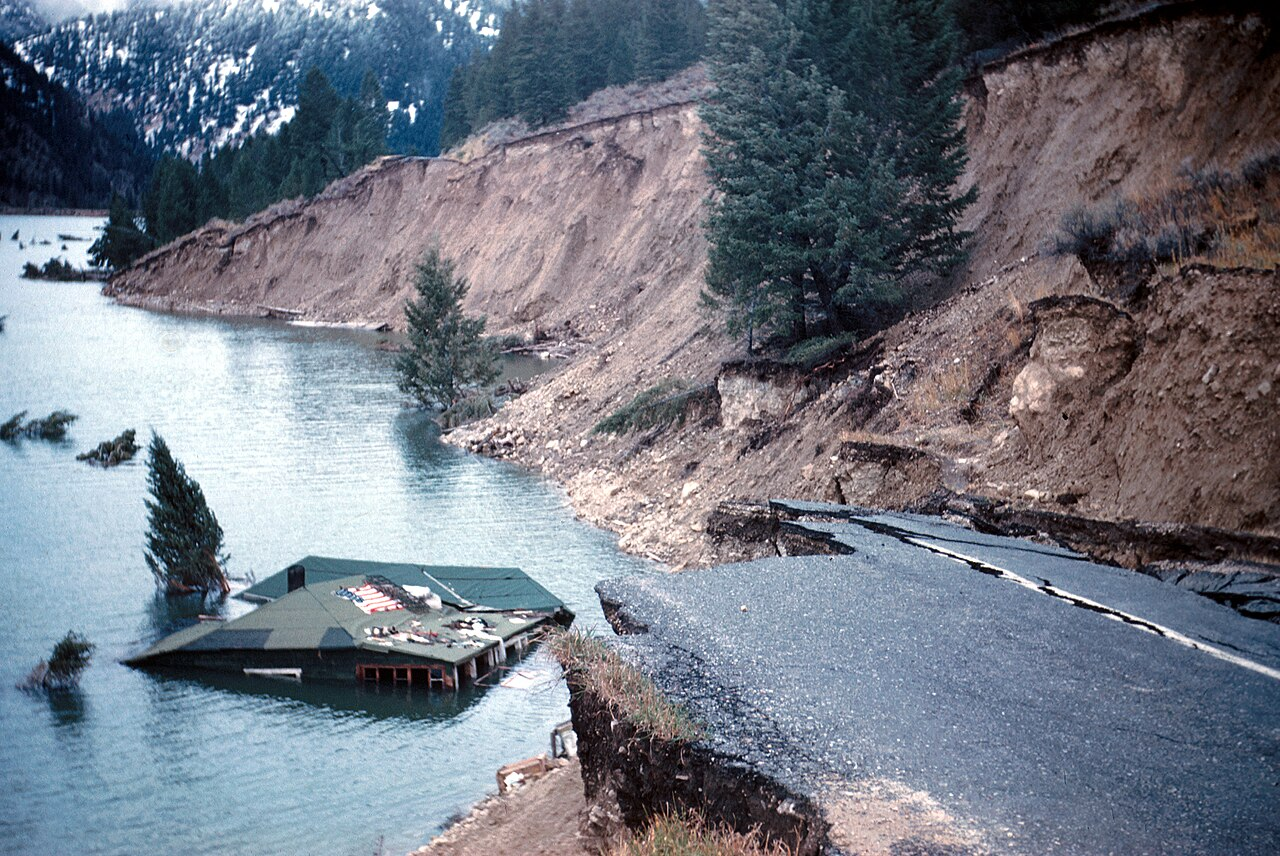
\includegraphics[width=0.6\linewidth]{images/book1/g7-hebgen-road.jpg}

{\small हेबजेन \omterm{def:g1:landscapes-around-us:water}{झील} \omterm{def:g4:volcanoes-earthquakes-first-look:earthquake}{भूकंप} के बाद, मोंटाना (संयुक्त राज्य अमेरिका), अगस्त 1959:
\omterm{def:g1:landscapes-around-us:water}{झील} के किनारे वाली सड़क धँसकर पानी में चली गई, और एक लॉज लगभग पानी में डूब
गया। ऐसा नुकसान ऊँची \omterm{def:g7:earthquakes:intensity}{तीव्रता} की पहचान है। फ़ोटो: विटकाइंड, अमेरिकी
भूवैज्ञानिक सर्वेक्षण (सार्वजनिक डोमेन,
विकिमीडिया कॉमन्स के ज़रिए)।}
% ledger: commons:hebgen-road, usgs:mmi
\label{fig:g7:earthquakes:hebgen}
\end{omfigure}

\section{सुनामी}

\begin{definition}[सुनामी]\label{def:g7:earthquakes:tsunami}
\emph{सुनामी}\index{सुनामी} \omterm{def:g2:water-on-earth:ocean}{समुद्र} की लहरों की एक श्रृंखला है जो \omterm{def:g2:water-on-earth:ocean}{समुद्र} की तली की
अचानक गति से पैदा होती है --- आमतौर पर \omterm{def:g2:water-on-earth:ocean}{समुद्र} के नीचे के \omterm{def:g4:volcanoes-earthquakes-first-look:earthquake}{भूकंप} से, कभी-कभी किसी
\omterm{def:g4:volcanoes-earthquakes-first-look:eruption}{उद्गार} से --- और जो पूरे \omterm{def:g2:water-on-earth:ocean}{महासागर} पार करके तटों को
डुबो सकती है।
\end{definition}

जब \omterm{def:g2:water-on-earth:ocean}{समुद्र} के नीचे कोई \omterm{def:g7:earthquakes:fault}{भ्रंश} टूटता है, तो \omterm{def:g2:water-on-earth:ocean}{समुद्र} की तली अचानक ऊपर या नीचे खिसकती
है, और अपने ऊपर के पानी के पूरे स्तंभ को उठा देती है या नीचे कर देती है। पानी लहरों में फैल जाता है। खुले गहरे \omterm{def:g2:water-on-earth:ocean}{महासागर} में \omterm{def:g7:earthquakes:tsunami}{सुनामी}
हैरान करती है: वह शायद ही कभी एक मीटर से ज़्यादा ऊँची होती है, और जहाज़ों को पता
भी नहीं चलता कि वह उनके नीचे से गुज़री। पर वह तेज़ होती है: \qty{800}{km/h} से
ज़्यादा, जेट विमान जितनी तेज़। \omterm{def:g1:landscapes-around-us:water}{तट} के पास उथले पानी में पहुँचने पर वह धीमी होकर 30
या \qty{50}{km/h} पर आ जाती है --- अब भी किसी के दौड़ने से तेज़ --- और ऊँची होती
जाती है। ज़्यादातर \omterm{def:g7:earthquakes:tsunami}{सुनामी} \omterm{def:g1:landscapes-around-us:water}{तट} पर \qty{3}{m} से कम ऊँची होती हैं; सबसे बड़ी
\qty{30}{m} पार कर जाती हैं। पहली लहर हमेशा सबसे बड़ी नहीं होती, और लहरें घंटों तक
आती रह सकती हैं।
% ledger: nws:tsunami-speed, nws:tsunami-safety

\begin{omfigure}
\begin{tikzpicture}[font=\small, x=1cm, y=1cm]
  % sea floor profile: deep ocean on the left, shelf and coast on the right
  \fill[omSea!35] (0,0) -- (13.2,0) -- (13.2,-0.2) -- (11.4,-0.45) -- (10.2,-1.0) -- (8.8,-2.6) -- (0,-2.6) -- cycle;
  \fill[brown!35] (0,-2.6) -- (8.8,-2.6) -- (10.2,-1.0) -- (11.4,-0.45) -- (13.2,-0.2) -- (13.2,0.5) -- (14.2,1.0) -- (14.2,-3.3) -- (0,-3.3) -- cycle;
  % the broken fault under the sea, at left; one block lifted
  \draw[very thick, red!70!black] (1.9,-3.3) -- (2.3,-2.6);
  \draw[-{Stealth[length=2mm]}, thick] (2.75,-3.1) -- (2.75,-2.75);
  \node[anchor=north west, font=\footnotesize, red!70!black] at (0.1,-3.35) {भ्रंश टूटता है, समुद्र की तली उछलती है};
  % wave: low and long in the deep ocean, short and tall near the coast
  \draw[blue!70!black, thick] (0,0) .. controls (1.2,0.18) and (2.2,0.18) .. (3.4,0)
     -- (5.0,0) .. controls (5.8,0.12) and (6.6,0.12) .. (7.4,0) -- (10.6,0)
     .. controls (11.0,0.55) and (11.6,0.9) .. (12.1,0) -- (13.2,0);
  \node[align=center, font=\footnotesize] at (2.0,0.85) {गहरा महासागर: लगभग 1 मी ऊँची,\\800 किमी/घंटा से ज़्यादा};
  \node[align=center, font=\footnotesize] at (11.1,1.55) {तट के पास: धीमी\\(30 से 50 किमी/घंटा), कहीं ज़्यादा ऊँची};
  \draw[-{Stealth[length=2.5mm]}, thick, blue!70!black] (4.4,0.45) -- (6.4,0.45);
  \node[font=\footnotesize] at (6.0,-1.5) {हज़ारों मीटर गहरा};
  \node[font=\footnotesize] at (12.0,-0.75) {उथला};
\end{tikzpicture}

{\small \omterm{def:g2:water-on-earth:ocean}{महासागर} पार करती एक \omterm{def:g7:earthquakes:tsunami}{सुनामी} (एक चित्र, पैमाने पर नहीं: लहर की ऊँचाई बहुत
बढ़ाकर दिखाई गई है)। गहरे \omterm{def:g2:water-on-earth:ocean}{महासागर} के ऊपर वह नीची और बहुत तेज़ होती है; \omterm{def:g1:landscapes-around-us:water}{तट} के पास
उथले पानी में वह धीमी होकर ऊँची हो जाती है।}
% ledger: nws:tsunami-speed
\label{fig:g7:earthquakes:tsunami}
\end{omfigure}

\begin{example}[सुमात्रा से श्रीलंका तक]\label{ex:g7:earthquakes:colombo}
श्रीलंका का सबसे बड़ा शहर कोलंबो 2004 के \omterm{def:g4:volcanoes-earthquakes-first-look:earthquake}{भूकंप} के \omterm{def:g7:earthquakes:focus}{अधिकेंद्र} से लगभग
\qty{1830}{km} दूर है। \qty{800}{km/h} पर \omterm{def:g7:earthquakes:tsunami}{सुनामी} यह दूरी
$1830 \div 800 \approx 2.3$~घंटे में तय करती है, यानी लगभग 2~घंटे
17~मिनट में। श्रीलंका में किसी ने \omterm{def:g4:volcanoes-earthquakes-first-look:earthquake}{भूकंप} महसूस नहीं किया: लहर बिना किसी चेतावनी के
आई, सिवाय ख़ुद \omterm{def:g2:water-on-earth:ocean}{समुद्र} के।
% ledger: nws:tsunami-speed, usgs:largest (distance and time in figdata/grade-7/quake_counts.py, part tsunami)
\end{example}

\begin{remark}[समुद्र की दी हुई चेतावनी]\label{rem:g7:earthquakes:natural-warning}
% ledger: nws:tsunami-natural-warning, nws:tsunami-speed, shakeout:dch
\omterm{def:g1:landscapes-around-us:water}{तट} पर तीन संकेत \omterm{def:g7:earthquakes:tsunami}{सुनामी} की सूचना दे सकते हैं: एक तेज़ या लंबा \omterm{def:g4:volcanoes-earthquakes-first-look:earthquake}{भूकंप}; \omterm{def:g2:water-on-earth:ocean}{समुद्र} का
अजीब बर्ताव --- अचानक \omterm{def:g5:water-shapes-the-land:flood}{बाढ़}, या पानी का \omterm{def:g1:landscapes-around-us:water}{तट} से बहुत दूर तक पीछे हट जाना, जिससे
बहुत नीचे भाटे की तरह \omterm{def:g2:water-on-earth:ocean}{समुद्र} की तली दिखने लगे; या \omterm{def:g2:water-on-earth:ocean}{महासागर} से आती तेज़ गर्जना।
काँपने के दौरान, जैसा तुमने सीखा है वैसे अपना बचाव करो (झुको, ढको, पकड़े रहो)।
फिर किसी आधिकारिक चेतावनी का इंतज़ार मत करो: तुरंत जितना ऊँचा, या ज़मीन के अंदर
जितना दूर, जा सको, जाओ। पास के \omterm{def:g4:volcanoes-earthquakes-first-look:earthquake}{भूकंप} से उठी \omterm{def:g7:earthquakes:tsunami}{सुनामी} कुछ ही मिनटों में
पहुँच सकती है।
\end{remark}


\section{अभ्यास}

\begin{exercise}[$\star$]\label{exo:g7:earthquakes:1}
हर शब्द को उसके अर्थ से मिलाओ: \omterm{def:g7:earthquakes:fault}{भ्रंश}; \omterm{def:g7:earthquakes:focus}{भूकंप-मूल}; \omterm{def:g7:earthquakes:focus}{अधिकेंद्र}; \omterm{def:g7:earthquakes:seismometer}{भूकंपमापी}; \omterm{def:g7:earthquakes:magnitude}{परिमाण};
\omterm{def:g7:earthquakes:intensity}{तीव्रता}। (क) ज़मीन के नीचे वह जगह जहाँ फिसलन शुरू होती है। (ख) किसी एक जगह पर
ज़मीन कितनी ज़ोर से काँपी। (ग) \omterm{def:g3:stones-pebbles-sand:rock}{चट्टानों} में एक दरार जिसके साथ-साथ दोनों ओर के
हिस्से खिसके हैं। (घ) \omterm{def:g7:earthquakes:focus}{भूकंप-मूल} के ऊपर सतह पर का बिंदु। (ङ) \omterm{def:g4:volcanoes-earthquakes-first-look:earthquake}{भूकंप} का आकार, हर
\omterm{def:g4:volcanoes-earthquakes-first-look:earthquake}{भूकंप} के लिए एक संख्या। (च) एक उपकरण जो ज़मीन के काँपने को दर्ज
करता है।
\end{exercise}

\begin{exercise}[$\star$]\label{exo:g7:earthquakes:2}
किसी \omterm{def:g4:volcanoes-earthquakes-first-look:earthquake}{भूकंप} का \omterm{def:g7:earthquakes:focus}{भूकंप-मूल} एक गाँव के ठीक \qty{30}{km} नीचे है।
(क) \omterm{def:g7:earthquakes:focus}{अधिकेंद्र} कहाँ है? (ख) गाँव \omterm{def:g7:earthquakes:focus}{भूकंप-मूल} से कितनी दूर है? (ग) एक दूसरा गाँव
\omterm{def:g7:earthquakes:focus}{अधिकेंद्र} से \qty{40}{km} दूर है। क्या वहाँ \omterm{def:g7:earthquakes:intensity}{तीव्रता} आमतौर पर पहले गाँव से ज़्यादा
होगी या कम? क्यों?
\end{exercise}

\begin{exercise}[$\star$]\label{exo:g7:earthquakes:3}
\omterm{def:g7:earthquakes:magnitude}{परिमाण} या \omterm{def:g7:earthquakes:intensity}{तीव्रता}? (क) ``\omterm{def:g4:volcanoes-earthquakes-first-look:earthquake}{भूकंप} 6.8 मापा गया।'' (ख) ``हमारी गली में सारे बर्तन
गिर गए और एक चिमनी टूट गई।'' (ग) ``शहर में यह VI था और \omterm{def:g1:landscapes-around-us:landform}{पहाड़ियों} के गाँवों में
IV।'' (घ) ``इसने पिछले साल वाले से
32~गुना ज़्यादा ऊर्जा छोड़ी।''
\end{exercise}

\begin{exercise}[$\star$]\label{exo:g7:earthquakes:4}
सही या ग़लत? ग़लत वाक्यों को सुधारो। (क) वैज्ञानिक एक हफ़्ता पहले बता सकते हैं कि
\omterm{def:g4:volcanoes-earthquakes-first-look:earthquake}{भूकंप} कब आएगा। (ख) खुले \omterm{def:g2:water-on-earth:ocean}{महासागर} में \omterm{def:g7:earthquakes:tsunami}{सुनामी} पानी की एक विशाल दीवार होती है।
(ग) एक \omterm{def:g4:volcanoes-earthquakes-first-look:earthquake}{भूकंप} का एक ही \omterm{def:g7:earthquakes:magnitude}{परिमाण} पर बहुत-सी \omterm{def:g7:earthquakes:intensity}{तीव्रताएँ} होती हैं। (घ) ज़्यादातर बड़े
\omterm{def:g4:volcanoes-earthquakes-first-look:earthquake}{भूकंप} \omterm{def:g7:plate-tectonics:plate-boundary}{प्लेट सीमाओं} के पास आते हैं।
\end{exercise}

\begin{exercise}[$\star\star$]\label{exo:g7:earthquakes:5}
प्रति वर्ष \omterm{def:g4:volcanoes-earthquakes-first-look:earthquake}{भूकंपों} वाले आलेख का उपयोग करो। (क) एक वर्ष में \omterm{def:g7:earthquakes:magnitude}{परिमाण} 6 से 6.9 के
लगभग कितने \omterm{def:g4:volcanoes-earthquakes-first-look:earthquake}{भूकंप} आते हैं? और \omterm{def:g7:earthquakes:magnitude}{परिमाण} 7 से 7.9 के? (ख) दूसरे वाले पहले वालों से
कितने गुना कम हैं? (ग) 7 और उससे ऊपर के तीनों दंडों को जोड़ो: एक वर्ष में \omterm{def:g7:earthquakes:magnitude}{परिमाण}
7 या उससे ज़्यादा के लगभग कितने \omterm{def:g4:volcanoes-earthquakes-first-look:earthquake}{भूकंप} आते हैं? (घ) आलेख \omterm{def:g7:earthquakes:magnitude}{परिमाण} 9 या उससे ज़्यादा
के लिए प्रति वर्ष 0.04 बताता है। 50~वर्षों में यह
कितने हुए?
\end{exercise}

\begin{exercise}[$\star\star$]\label{exo:g7:earthquakes:6}
\omterm{def:g7:earthquakes:magnitude}{परिमाणों} की तुलना वाली विधि का उपयोग करो। (क) \omterm{def:g7:earthquakes:magnitude}{परिमाण} 7 का \omterm{def:g4:volcanoes-earthquakes-first-look:earthquake}{भूकंप} \omterm{def:g7:earthquakes:magnitude}{परिमाण} 6 वाले से
कितने गुना ज़्यादा ऊर्जा छोड़ता है? (ख) और \omterm{def:g7:earthquakes:magnitude}{परिमाण} 8 वाला \omterm{def:g7:earthquakes:magnitude}{परिमाण} 6 वाले से? (ग)
उसी दूरी पर, \omterm{def:g7:earthquakes:magnitude}{परिमाण} 6 और 8 के बीच, \omterm{def:g7:earthquakes:seismometer}{भूकंपलेख} पर तरंगें
कितने गुना बड़ी होती हैं?
\end{exercise}

\begin{exercise}[$\star\star$]\label{exo:g7:earthquakes:7}
तेज़ और धीमी तरंगों के बीच देरी के हर सेकंड के लिए \qty{8}{km} लो। (क) एक स्टेशन
\qty{5}{s} की देरी दर्ज करता है। \omterm{def:g4:volcanoes-earthquakes-first-look:earthquake}{भूकंप} कितनी दूर था? (ख) दूसरा स्टेशन
\qty{25}{s} दर्ज करता है। (ग) एक \omterm{def:g4:volcanoes-earthquakes-first-look:earthquake}{भूकंप} किसी स्टेशन से \qty{120}{km} दूर आया: वह
स्टेशन कितनी देरी पढ़ेगा? (घ) अकेला एक स्टेशन यह क्यों नहीं बता सकता कि \omterm{def:g7:earthquakes:focus}{अधिकेंद्र}
कहाँ है?
\end{exercise}

\begin{exercise}[$\star\star$]\label{exo:g7:earthquakes:8}
\omterm{def:g7:earthquakes:intensity}{तीव्रता} वाली तालिका का उपयोग करो। हर रिपोर्ट के लिए \omterm{def:g7:earthquakes:intensity}{तीव्रता} बताओ। (क) ``लगभग
सबको महसूस हुआ; हम जाग गए और दो गिलास टूट गए।'' (ख) ``केवल ऊपर की मंज़िल पर
आराम कर रही मेरी दादी को महसूस हुआ; लैंप झूल गया।'' (ग) ``दीवारें और चिमनियाँ
गिर गईं; कई घर आंशिक रूप से ढह गए।'' (घ) एक ही \omterm{def:g4:volcanoes-earthquakes-first-look:earthquake}{भूकंप} से रिपोर्ट (क) और (ग)
मिलीं। समझाओ कि यह कैसे संभव है।
\end{exercise}

\begin{exercise}[$\star\star$]\label{exo:g7:earthquakes:9}
1976--2025 के \omterm{def:g7:earthquakes:magnitude}{परिमाण}~6 या उससे ज़्यादा के 7\,031 \omterm{def:g4:volcanoes-earthquakes-first-look:earthquake}{भूकंपों} में से 5\,561 का
\omterm{def:g7:earthquakes:focus}{भूकंप-मूल} \qty{70}{km} से कम गहरा था। (क) कितनों का \omterm{def:g7:earthquakes:focus}{भूकंप-मूल} ज़्यादा गहरा था?
(ख) यह कितना प्रतिशत है? निकटतम पूर्ण संख्या तक पूर्णांकित करो। (ग) गहरे \omterm{def:g4:volcanoes-earthquakes-first-look:earthquake}{भूकंप} वहाँ
आते हैं जहाँ एक \omterm{def:g7:plate-tectonics:plate}{प्लेट} दूसरी के नीचे धँसती है। समझाओ कि वहाँ वे इतनी गहराई पर
क्यों शुरू हो सकते हैं।
\end{exercise}

\begin{exercise}[$\star\star$]\label{exo:g7:earthquakes:10}
मालदीव की राजधानी माले 2004 के \omterm{def:g4:volcanoes-earthquakes-first-look:earthquake}{भूकंप} के \omterm{def:g7:earthquakes:focus}{अधिकेंद्र} से लगभग \qty{2500}{km} दूर
है। (क) \qty{800}{km/h} पर \omterm{def:g7:earthquakes:tsunami}{सुनामी} को वहाँ पहुँचने में कितना समय लगा? घंटे और
मिनट बताओ। (ख) वह कोलंबो (2~घंटे 17~मिनट) से कितनी देर बाद पहुँची? (ग) ऐसी
देरियों के साथ, एक चेतावनी प्रणाली बहुत-सी जानें क्यों बचा सकती
थी?
\end{exercise}

\begin{exercise}[$\star\star\star$]\label{exo:g7:earthquakes:11}
एक \omterm{def:g7:earthquakes:tsunami}{सुनामी} \qty{800}{km/h} पर \qty{400}{km} गहरा \omterm{def:g2:water-on-earth:ocean}{महासागर} पार करती है, फिर
\qty{40}{km/h} पर उथले पानी के आख़िरी \qty{20}{km}। (क) गहरे हिस्से के लिए उसे
कितने मिनट लगते हैं? (ख) उथले हिस्से के लिए? (ग) पूरी यात्रा कितनी लंबी है?
(घ) तुम्हारे जवाबों में हैरानी की क्या बात है? (ङ) धीमी होने पर लहर ऊँची क्यों
होती जाती है?
\end{exercise}

\begin{exercise}[$\star\star\star$]\label{exo:g7:earthquakes:12}
(क) \omterm{def:g7:earthquakes:magnitude}{परिमाण} 9 का \omterm{def:g4:volcanoes-earthquakes-first-look:earthquake}{भूकंप} \omterm{def:g7:earthquakes:magnitude}{परिमाण} 6 वाले से कितने गुना ज़्यादा ऊर्जा छोड़ता है? (ख) हर
वर्ष \omterm{def:g7:earthquakes:magnitude}{परिमाण} 6 से 6.9 के लगभग 127 \omterm{def:g4:volcanoes-earthquakes-first-look:earthquake}{भूकंप} आते हैं। मान लो उनमें से हर एक \omterm{def:g7:earthquakes:magnitude}{परिमाण} 6
जितनी ऊर्जा छोड़ता है। \omterm{def:g7:earthquakes:magnitude}{परिमाण}~9 के एक \omterm{def:g4:volcanoes-earthquakes-first-look:earthquake}{भूकंप} जितनी ऊर्जा छोड़ने में उनके कितने
वर्ष लगते हैं? (ग) इससे सबसे बड़े \omterm{def:g4:volcanoes-earthquakes-first-look:earthquake}{भूकंपों} द्वारा ले जाई गई ऊर्जा के हिस्से के बारे
में क्या पता चलता है?
\end{exercise}

\section{समस्या: ज़मीन कहाँ काँपी?}

\begin{problem}[{सप्ताहांत समस्या --- तीन स्टेशन समुद्र के नीचे के एक भूकंप को दर्ज
करते हैं, मानचित्र पर अधिकेंद्र ढूँढा जाता है, और सुनामी पहुँचने से पहले पोर्ट हेल
शहर को चेतावनी दी जाती है}]
\label{pb:g7:earthquakes:1}
% ledger: nws:tsunami-speed, usgs:seismograph, data:prem (figdata/grade-7/epicentre.py)
एक काल्पनिक \omterm{def:g1:landscapes-around-us:water}{तट} के \omterm{def:g2:water-on-earth:ocean}{समुद्र} के नीचे एक \omterm{def:g4:volcanoes-earthquakes-first-look:earthquake}{भूकंप} आता है। तीन \omterm{def:g7:earthquakes:seismometer}{भूकंपमापी} स्टेशन, A, B
और C, ज़मीन पर हैं; पोर्ट हेल शहर एक द्वीप पर है (नीचे \omterm{def:g2:drawing-to-map:map}{मानचित्र}; एक वर्ग
\qty{20}{km} है)। इस क्षेत्र में तेज़ और धीमी तरंगों के बीच देरी का हर सेकंड
\qty{8}{km} दर्शाता है। स्टेशन यह
दर्ज करते हैं:

\begin{center}
\small
\begin{tabular}{|c|c|c|}
\hline
\textbf{स्टेशन} & \textbf{तेज़ तरंगें पहुँचती हैं} & \textbf{धीमी तरंगें पहुँचती हैं} \\
\hline
A & 10:15:25 & 10:15:45 \\
B & 10:15:16 & 10:15:29 \\
C & 10:15:19 & 10:15:34 \\
\hline
\end{tabular}
\end{center}

\medskip
\noindent\textbf{भाग I --- तीन स्टेशन।}\par\nopagebreak
\begin{enumerate}[beginpenalty=10000]
  \item हर स्टेशन के लिए दोनों के पहुँचने के बीच की देरी सेकंड में
        निकालो।
  \item कौन-सा स्टेशन \omterm{def:g4:volcanoes-earthquakes-first-look:earthquake}{भूकंप} के सबसे पास है? बिना किसी गणना के तुम यह कैसे बता
        सकते हो?
  \item हर स्टेशन से \omterm{def:g4:volcanoes-earthquakes-first-look:earthquake}{भूकंप} की दूरी निकालो।
  \item केवल स्टेशन A की दूरी से यह पता नहीं चलता कि \omterm{def:g4:volcanoes-earthquakes-first-look:earthquake}{भूकंप} कहाँ था। उन सभी
        जगहों का वर्णन करो जो A से इस दूरी पर हैं।
\end{enumerate}

\begin{center}
\begin{tikzpicture}
  \begin{axis}[axis equal image, width=12cm, xmin=-60, xmax=360, ymin=-200, ymax=260,
      xtick={-60,-40,...,360}, ytick={-200,-180,...,260}, xticklabels={}, yticklabels={},
      major tick length=0pt,
      axis background/.style={fill=omSea!25}, clip mode=individual]
    \addplot[fill=omLithAlluv, draw=black!50, line width=0.4pt] table[x=x, y=y] {figdata/out/grade-7-epicentre-p-west.dat};
    \addplot[fill=omLithAlluv, draw=black!50, line width=0.4pt] table[x=x, y=y] {figdata/out/grade-7-epicentre-p-north.dat};
    \addplot[fill=omLithAlluv, draw=black!50, line width=0.4pt] table[x=x, y=y] {figdata/out/grade-7-epicentre-p-island.dat};
    % the grid over land and sea, drawn before the labels
    \pgfplotsinvokeforeach{-40,-20,...,340}{\draw[black!15] (axis cs:#1,-200) -- (axis cs:#1,260);}
    \pgfplotsinvokeforeach{-180,-160,...,240}{\draw[black!15] (axis cs:-60,#1) -- (axis cs:360,#1);}
    \addplot[only marks, mark=triangle*, mark size=3.2pt, black,
        nodes near coords, point meta=explicit symbolic,
        nodes near coords style={font=\small\bfseries, anchor=south west}]
      table[x=x, y=y, meta=name] {figdata/out/grade-7-epicentre-p-stations.dat};
    \addplot[only marks, mark=square*, mark size=2.4pt, red!70!black]
      table[x=x, y=y] {figdata/out/grade-7-epicentre-p-town.dat};
    \node[font=\small, anchor=north east, fill=omSea!25, inner sep=1pt] at (axis cs:264,-102) {पोर्ट हेल};
    \draw[-{Stealth[length=2.5mm]}, line width=0.8pt] (axis cs:330,200) -- (axis cs:330,245);
    \node[font=\scriptsize\bfseries, anchor=north] at (axis cs:330,200) {उ};
    \node[font=\scriptsize, anchor=west, fill=omLithAlluv, inner sep=1pt] at (axis cs:170,240) {1 वर्ग = 20 km};
    \fill (axis cs:-60,-200) circle (1.5pt);
    \node[font=\small\bfseries, anchor=north east] at (axis cs:-60,-200) {O};
  \end{axis}
\end{tikzpicture}
\end{center}
% ledger: (invented map: figdata/grade-7/epicentre.py, parts p-west, p-north, p-island, p-stations, p-town)

\medskip
\noindent\textbf{भाग II --- अधिकेंद्र ढूँढना।}\par\nopagebreak
\begin{enumerate}[resume, beginpenalty=10000]
  \item एक वर्ग \qty{20}{km} है। हर वृत्त की त्रिज्या कितने वर्ग
        है?
  \item कोना O \omterm{def:g2:drawing-to-map:map}{मानचित्र} के नीचे बाईं ओर रखो। स्टेशन C, O से 3~वर्ग पूर्व और
        14.5~वर्ग उत्तर में है; C से ठीक पूर्व की ओर 6~वर्ग
        (\qty{120}{km}) जाने पर तुम एक बिंदु~E पर पहुँचते हो। \omterm{def:g2:drawing-to-map:map}{मानचित्र} पर जाँचो
        कि E, A और B के वृत्तों पर भी है: यही \omterm{def:g7:earthquakes:focus}{अधिकेंद्र} है।
        यह O से कितने वर्ग पूर्व और उत्तर में है?
  \item \omterm{def:g7:earthquakes:focus}{अधिकेंद्र} ज़मीन पर है या \omterm{def:g2:water-on-earth:ocean}{समुद्र} के नीचे? इससे क्या फ़र्क़ पड़ता है?
  \item \omterm{def:g7:earthquakes:magnitude}{परिमाण} 7.4 था। इसने \omterm{def:g7:earthquakes:magnitude}{परिमाण}~6.4 के \omterm{def:g4:volcanoes-earthquakes-first-look:earthquake}{भूकंप} से कितने गुना ज़्यादा ऊर्जा
        छोड़ी?
\end{enumerate}

\medskip
\noindent\textbf{भाग III --- लहर तट तक पहुँचती है।}\par\nopagebreak
\begin{enumerate}[resume, beginpenalty=10000]
  \item \omterm{def:g2:drawing-to-map:map}{मानचित्र} पर पोर्ट हेल \omterm{def:g7:earthquakes:focus}{अधिकेंद्र} से 12~वर्ग दूर है। यह कितने
        किलोमीटर है?
  \item \qty{800}{km/h} पर \omterm{def:g7:earthquakes:tsunami}{सुनामी} को पोर्ट हेल तक पहुँचने में कितने मिनट लगते
        हैं?
  \item \omterm{def:g4:volcanoes-earthquakes-first-look:earthquake}{भूकंप} का पता लगाने और चेतावनी भेजने में काँपना शुरू होने के बाद
        5~मिनट लगते हैं। \omterm{def:g4:volcanoes-earthquakes-first-look:earthquake}{भूकंप} के कितने समय बाद चेतावनी पोर्ट हेल तक पहुँचती है?
  \item \omterm{def:g7:earthquakes:tsunami}{सुनामी} पहुँचने से पहले पोर्ट हेल के लोगों के पास ऊँची ज़मीन तक पहुँचने के
        लिए कितने मिनट हैं?
\end{enumerate}
\end{problem}
